%&template
\documentclass{article}
\usepackage{src/template}

\endofdump
\usepackage{minted}

\date{2026 -- 01 -- 18}
\useTemplate[NPA, Exercise=11]
\title{NPA -- Exercise 11}


\begin{document}
\maketitle
    
    \section{}

        \begin{figure}[h]
        \centering
        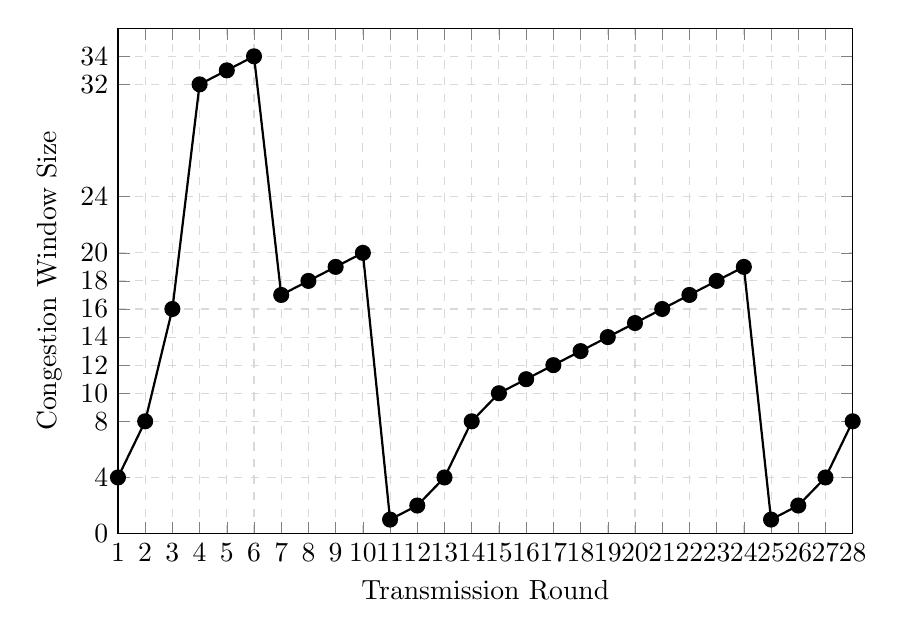
\begin{tikzpicture}
        \begin{axis}[
            width=0.9\textwidth,
            height=8cm,
            xlabel={Transmission Round},
            ylabel={Congestion Window Size},
            xmin=1, xmax=28,
            ymin=0, ymax=36,
            xtick={1,2,3,4,5,6,7,8,9,10,11,12,13,14,15,16,17,18,19,20,21,22,23,24,25,26,27,28},
            ytick={0,4,8,10,12,14,16,18,20,24,32,34},
            grid=both,
            grid style={dashed,gray!30},
            mark size=2.5pt
        ]
        
        \addplot[
            mark=*,
            thick
        ] coordinates {
            (1,4) (2,8) (3,16) (4,32)
            (5,33) (6,34)
            (7,17) (8,18) (9,19) (10,20)
            (11,1) (12,2) (13,4) (14,8)
            (15,10) (16,11) (17,12) (18,13)
            (19,14) (20,15) (21,16) (22,17)
            (23,18) (24,19)
            (25,1) (26,2) (27,4) (28,8)
        };
        
        \end{axis}
        \end{tikzpicture}
        \caption{Congestion Window, taken from the task sheet 11.}
        \label{fig:tcp-reno-cwnd}
        \end{figure}
    
    \subsection{}

        In the first round, we can see from the diagram that the congestion window is 4.

    \subsection{}

        In TCP Reno, slow start describes the doubling of the congestion window. This behavior can be seen in the diagram at the following intervals:

        \begin{tabular}{l l l l}
            Transmission Round:  & 1 & $\xrightarrow{}$  & 4 \\
            Transmission Round:  & 11 & $\xrightarrow{}$ & 14 \\
            Transmission Round:  & 25 & $\xrightarrow{}$ & 28
        \end{tabular}
    
    \subsection{}

        Congestion avoidance describes the linear increase of the congestion window by 1. This can be seen in the following intervals in the diagram:

        \begin{tabular}{l l l l}
            Transmission Round:  & 5 & $\xrightarrow{}$  & 6 \\
            Transmission Round:  & 7 & $\xrightarrow{}$ & 10 \\
            Transmission Round:  & 15 & $\xrightarrow{}$ & 24
        \end{tabular}

        In round 4, the window size is 32 and has therefore reached the threshold value. Congestion avoidance only begins after this point. This means that the first interval is only from 5 to 6, even though the increase from 4 to 6 is linear.

    \subsection{} \label{excercise d}

        In the event of a timeout and thus a suspected serious error, the window is set to 1. In round 6, the window is only halved, so this must be a triple dup ACK.

    \subsection{}

        In relation to \ref{excercise d}, the window was set to 1 at round 10, which means that a timeout must have been detected.
    
    \subsection{}

        From the first round to the fourth, the transmission is in slow start mode, so in the fourth round, the window size was set equal to the threshold value. Accordingly, the threshold value in the first round is 32.
        
    \subsection{}

        Before the 8th round, there was a triple dup ACK error at window size 34. Accordingly, the threshold value was halved to 17 and the window size was also set to the threshold value, i.e., 17. At time 8, there was no further error, so the threshold value remains at 17.

    \subsection{}

        Before round 12, there was another packet loss, which affected the threshold value. With WindowSize 20, a timeout occurred, which is why the window size was set to 1, but the threshold value was only halved to 10. This makes sense because a timeout indicates a complete loss of connection and the transmission speed should not be affected after the connection is reestablished. The threshold value for round 12 is therefore 10.

    \subsection{}

        The number of segments sent is the cumulative number of window sizes per round. Up to round 3, $4 + 8 + 16 = 28$ segments were sent, which is why the 30th was transferred to the fourth round. We can say this in our example because no error has occurred up to this point.
    
    \subsection{}

        For round 28, the window size is 8. With a triple duplicate ACK, the threshold value is halved, resulting in 4, and the window size is set to the threshold value, also resulting in 4. Compare with task \ref{excercise d}

    \section{}

 \subsection{}

 Highlighted collection gets 10 Mbit/s.\\
 Reson: Bottleneck on Link 5 where all flows get 10 Mbit/s.
 More BW avalable for flow on Links 1 and 3\\
 Other connections on Link 1 get (210-10)/2 = 100 Mbit/s.
 Reason: Link 2 and other links for the flows have 210 Mbit/s and only the two flows on these (except the short bit between Router A and Host A where all 3 of the same flows are present).


 \subsection{}

 Bottleneck on Link 5 - increase it so Flow gets 70 Mbit/s (cause of bottleneck on link one when all 3 flows have fair share).
 Care - Flows from link 4 also need to be satisfied on Link 5 so that they don't decrease BW of our flow.
 Flows from Link 4 need 30 Mbit/s. Our flow needs 70 Mbit/s. Together Link 5 needs to be increased to 100 Mbit/s

 No higher thorughput cause bottheneck on Link 1.

    \subsection{}
 In the beginning Flow is 10 Mbit/s and the other two 100 Mbit/s each.
 The other two get reduced to 70 Mbit/s with the Flow also getting 70 Mbit/s.
 Flow increased and thus other TCP flows on link 1 had to decrease to satisfy fairness.





    
    \section{}
    \subsection{}
    Additive Increase\\
    Describes the process of adding one additional packet per RTT until a packet loss is detected. As a result this traffic increases linearly. 
    
    Multiplicative Decrease\\
    Describes the process of halving the sending rate at each loss event.

    Using AIMD results in a sawtooth-like behavior. \\
    Fairness\\
    Fairness of TCP sessions means that each session with a maximum link capacity (R) should have the same R/K part of the bandwidth. In reality, that is often not the case, due to different RTTs and one device being able to spawn unlimited sessions. 

    \subsection{}
    %\todo{maybe use 12Mbits as 1}
    Both TCP Reno sessions should have 1/2 of the bandwidth (6Mbit/s). Due to the AIMD, both flows would increase until both have over 1/2 of bandwidth used, causing both to land around 1/4 of bandwidth (3Mbit/s). In the end, both should cycle through a bandwidth usage between 1/4 (3Mbit/s) and 1/2 (6Mbit/s). 
    
    \subsection{}
    Due to the constant UDP stream the overall 'fair' sessions would have 6 Mbits to share. UDP does not provide flow control, as a result will not respond to the packet loss. And keep sending its data at its predetermined capacity. 

    Both TCP sessions would suffer from it, resulting in a halved bandwith.
    As a result both sessions would use between 1.5 Mbits and 3 Mbits using AIMD.

    \subsection{}
    ECN uses the ECN bit in the IP layer and the C \& E bit marking in TCP to communicate congestion-related information. 
    The sender sends the packet through the network. The packet has the ECN bits set to 01. On its way to the receiver, one router experiences congestion. As a result, it sets the bits to 11.
    The receiver answers the packet and keeps the ECN bits set to 11. As a result, the sender receives the packet and can reduce the network throughput to remove congestions. 
    In later communication, the congestion marking will be removed if it resolves the congestion. 


    Advantage: \\
    The sender regulates traffic based on feedback from the receiver. This allows the network to be used evenly and adjust the network output to reduce congestion in a timely manner. 


\end{document}